\documentclass[10pt, xcolor=dvipsnames]{beamer} 
\usetheme{Madrid}
%\usetheme{Hannover}
%\usetheme{Warsaw}
% Pour passer d'un theme vert sympa à un thème bleu pâle:  \usecolortheme[named=OliveGreen]{structure}  -> \usecolortheme[named=OliveGreen]{seahorse}
%\usecolortheme[named=OliveGreen]{structure} 
\usecolortheme{whale}
\usepackage{tikz}
\usetikzlibrary{arrows}
\usepackage{moreverb} 
\usepackage{pgf,pgfarrows,pgfnodes,pgfautomata,pgfheaps,pgfshade}
\usepackage{amsmath,amssymb}
\usepackage{colortbl}
%\usepackage{beamerthemesplit}
\usepackage{graphics}
\usepackage{setspace}
\usepackage[scaled=0.9]{helvet}
\usepackage{amsmath,amssymb}
\usepackage[utf8]{inputenc}
\usepackage{colortbl}
%\usepackage[english]{babel}
\usepackage{xcolor}
\usepackage[utf8]{inputenc} % LaTeX, comprends les accents !
\usepackage[T1]{fontenc}      % Police contenant les caract�res fran�ais
\usepackage{geometry}         % D�finir les marges
\usepackage[francais]{babel}  % Placez ici une liste de langues, la
%\usepackage[authoryear,round]{natbib}
\usepackage{pifont}
\usepackage{times}
\setbeamercovered{dynamic}
\usepackage{verbatim}


\setbeamerfont{section in toc}{size=\small}

\mode<article> % only for the article version
{
  \usepackage{fullpage}
  \usepackage{hyperref}
}

\mode<presentation>
{
  \setbeamertemplate{background canvas}[vertical shading][bottom=red!10,top=blue!10]

  \usefonttheme[onlysmall]{structurebold}
}




\title[UNIX/Linux]{L'environnement UNIX/Linux: un système d'exploitation pour la bioinformatique}
\author{%
  D. Puthier\inst{1}}
\institute[Inserm U1090/TAGC]{
  \inst{1}%
  http://pedagogix-tagc.univ-mrs.fr/courses/jgb53d-bd-prog/\\
  Inserm U1090 \\
  Technologies Avancées pour le Génome et la Clinique}
\date[2014]{}
\subject{UNIX/Linux}






\begin{document}
\maketitle
\begin{frame}
\frametitle{PLAN}
\begin{scriptsize}
\tableofcontents[currentsection, sectionstyle=show, hideallsubsections]
\end{scriptsize}
% \begin{itemize}
% \item Préambules.
% \item Commandes de base pour l'utilisation du shell.
% \item Fichiers et répertoires.
% \item Expressions régulières.
% \item Redirection.
% \item Les filtres.
% \item Quelques éléments pour la programmation.
% \item Contrôle des processus.
% \end{itemize}

\end{frame}




%=====================================================================================================================================================
%=====================================================================================================================================================
\section{Pourquoi UNIX/Linux ?}

\frame
{
%\setbeamercolor{block body}{bg=OliveGreen,fg=white}
\begin{block}{}
\begin{center}
\begin{huge}
Pourquoi UNIX/Linux ?
 \end{huge}
\end{center}
\end{block}

}





%*****************************************************************************************************************************************************
\subsection{Architecture d'un ordinateur}


\frame
{
\frametitle{Architecture d'un ordinateur}

  \begin{itemize}
  \item Composants d'un ordinateur
    \begin{itemize}
      \item Un micro-processeur (CPU, Central Process Unit): pour le traitement des données
      \item De la mémoire RAM (Random Access Memory, mémoire à accès aléatoire): stockage temporaire de l'information (données, programmes).
      \item Une mémoire morte (ROM ou Read-Only Memory): mémoire non volatile dans laquelle est stocké le BIOS (Basic Input Output System, permet le contrôle et l'intitialisation/contrôle des composants au démarrage).
      \item Des périphériques (disque dur pour stocker les programmes et les données, carte graphique,...).
      \item Des bus qui relient les éléments.
      \end{itemize}

  \end{itemize}
}


%*****************************************************************************************************************************************************
\subsection{Qu'est ce qu'un système d'exploitation ?}

\frame
{
\frametitle{Qu'est ce qu'un système d'exploitation ?}

%  \frametitle{Features of the Beamer Class}

  \begin{itemize}
  \item Assure les communications entre les ressources matérielles et les applications diverses (explorateur, traitement de texte,...).
         \begin{itemize}
            \item Programme -> requête vers OS (Operating system / système d'exploitation) -> pilote -> matériel.
            \item Limite la redondance (sinon chaque application devrait assurer l'interface avec le matériel)
         \end{itemize}
  \item Exemple de systèmes d'exploitation: Windows, Mac OS (Basé sur un système UNIX), Linux (Ubuntu, Debian, Opensuse...), Android (basé sur Linux), Chrome OS (basé sur Linux)...

  \end{itemize}
}


\subsection{UNIX/Linux: historique}
\frame
{
\frametitle{Historique}
\begin{itemize}
 \item Quelques repères chronologiques:
      \begin{itemize}
            \item 1969: Ken Thomson et Dennis Ritchie (Bell Labs AT\&T) développent UNIX. 
            \item 1973: 1ère version d'UNIX en langage C.
            \item 1978: Unix V7 (officielle).
            \item 1991: Freax (Linus Torvalds)
            \item 1994: Linux V1.0 (Intégre le noyau développé par Linus Torvalds et les outils GNU dévéloppés par Richard matthew Stallman).
            \item 1996: début du projet KDE d'interface graphique
            \item 1997: début du projet GNOME comme projet concurrent de KDE
      \end{itemize} 
\end{itemize}

}



\frame
{

  \begin{itemize}
  \item Constituants des systèmes Unix/Linux:
      \begin{itemize}
         \item le noyau (''kernel``): 
         \begin{itemize}                   
                   \item Gestion des processus (programmes).
                   \item Gestion de la mémoire
                   \item Gestion des entrées-sorties
                   \item Communication avec le matériel
           \end{itemize}
  \item La coquille  (''shell``): permet de donner des instructions au système d'exploitation.
  \item Le système de fichiers (FS, ''File System``): permet de stocker et d'organiser les fichiers.
 \end{itemize} 
\end{itemize}
}



%*****************************************************************************************************************************************************
\subsection{Pourquoi utiliser Linux en biologie ?}
\frame
    {
      \frametitle{Pourquoi utiliser Linux en biologie ?}
      
      \begin{itemize}
      \item Nécessité de manipuler des fichiers nombreux et volumineux.

	    \begin{itemize}
	    \item Comment ouvrir de tels fichiers sous Windows ?
	    \item Comment réaliser des actions simples sur ces fichiers (compter, filter, trier, ...)
	    \item Comment itérer sur ces fichiers avec Windows ?
	    \end{itemize}

      \item Nécéssité de réaliser des calculs nécessitant des serveurs puissants accessibles à distance.

        \begin{itemize}                   
        \item Système multi-utilisateurs, 
          \begin{itemize}
          \item Utilisateur standard (droits réduits)
          \item Super-utilisateur (root): tous les droits sur la machine.	
          \item Groupes (partage).
          \end{itemize}
		\end{itemize}

        \begin{itemize}                   
        \item Nombreux outils réseaux
          \begin{itemize}                   
          \item Nombreux outils de communication en réseau: FTP (File Transfert Protocol), SSH (Secure Shell), NFS (Network File System NFS),	...   
		  \end{itemize}	
		\end{itemize}

      \end{itemize}


    }

\subsection{Pourquoi utiliser Linux en biologie ?}
\frame
    {
      \frametitle{Pourquoi utiliser Linux en biologie ?}
      \begin{itemize}                   

      \item De nombreux logiciels développés spécifiquement pour les systèmes UNIX/Linux.
	  \item Nécessité de réaliser des ``pipelines de traitement''.
		\begin{itemize}
	    \item Possibilité de piloter la machine à travers des commandes unitaires pouvant être chaînées.        
          \begin{itemize}                   
          \item Création de scripts réalisant des tâches complexes.
          \end{itemize}
		\end{itemize}
      \item UNIX/Linux est le meilleur équipement pour la Bioinformatique (et bien d'autres choses)...

        \begin{itemize}                   
        \item Believe me...
        \end{itemize}
      \end{itemize}


    }

 

\subsection{Si vous souhaitez installer Linux}
\begin{frame}[fragile]
\frametitle{Si vous souhaitez installer Linux}
\begin{itemize}
\item De nombreuses ``Distributions'' disponibles (Ubuntu, Debian, RedHat, Opensuse, Mint...).
 \begin{itemize}
	\item Ubuntu: solution facile à prendre en main (de même que Mint).
	\item http://www.ubuntu.com/.
\item Solution 1: graver le CD, l'insérer, partitionner le disque* (-> dual boot) *
\item Solution 2: graver le CD. Utiliser VirtualBox (''virtualisation``, possibilité de lancer le système ubuntu depuis windows).
\end{itemize}
\end{itemize}

\scriptsize
* Préférable de faire une partition ''/`` et une partition ''/home``.
\normalsize
\end{frame}
 %=====================================================================================================================================================
 %=====================================================================================================================================================
% 
%\section{Notion de base pour l'utilisation de l'environnement UNIX/LINUX}
% 
% %*****************************************************************************************************************************************************

 %=====================================================================================================================================================
 %=====================================================================================================================================================

\section{Notions de base pour l'utilisation du shell}
\frame
{
%\setbeamercolor{block body}{bg=OliveGreen,fg=white}
\begin{block}{}
\begin{center}
\begin{huge}
Notions de base pour l'utilisation du shell
 \end{huge}
\end{center}
\end{block}

}

%*****************************************************************************************************************************************************

\subsection{Quelques bonnes habitudes}

\frame
    {
      \frametitle{Quelques bonnes habitudes}

      Remarque sur les noms des répertoires et fichiers:
      \begin{itemize}
      \item Uniquement des caractères alphanumériques et les caractères '-' et '\_'
        \begin{itemize}

        \item Pas d'espaces dans les noms. Eviter les caractères accentués et les caractères spéciaux.
        \end{itemize}

      \item Mettre une extension aux noms de fichiers permettant de deviner leurs types
        
        \begin{itemize}
        \item .txt pour un fichier de texte
        \item .sh pour un script shell
        \item .py pour un script Python
        \item ...
        \end{itemize}
      \item Attention: distinction entre les lettres majuscules et les lettres minuscules (sensible à la casse).

      \end{itemize}


    }



\subsection{Quelques bonnes habitudes}

\frame
    {
      \frametitle{Quelques bonnes habitudes}

      Remarque sur les noms des répertoires et fichiers:
      \begin{itemize}
      \item Uniquement des caractères alphanumériques et les caractères '-' et '\_'
        \begin{itemize}

        \item Pas d'espaces dans les noms. Eviter les caractères accentués et les caractères spéciaux.
        \end{itemize}

      \item Mettre une extension aux noms de fichiers permettant de deviner leurs types
        
        \begin{itemize}
        \item .txt pour un fichier de texte
        \item .sh pour un script shell
        \item .py pour un script Python
        \item ...
        \end{itemize}
      \item Attention: distinction entre les lettres majuscules et les lettres minuscules (sensible à la casse).

      \end{itemize}


    }


%*****************************************************************************************************************************************************


\subsection{Le terminal: Arghhh !!!}

\begin{frame}[fragile]
  
  \frametitle{Le terminal: Arghhh !!!}
  


    \begin{picture}(20,20)
  \put(35,-100){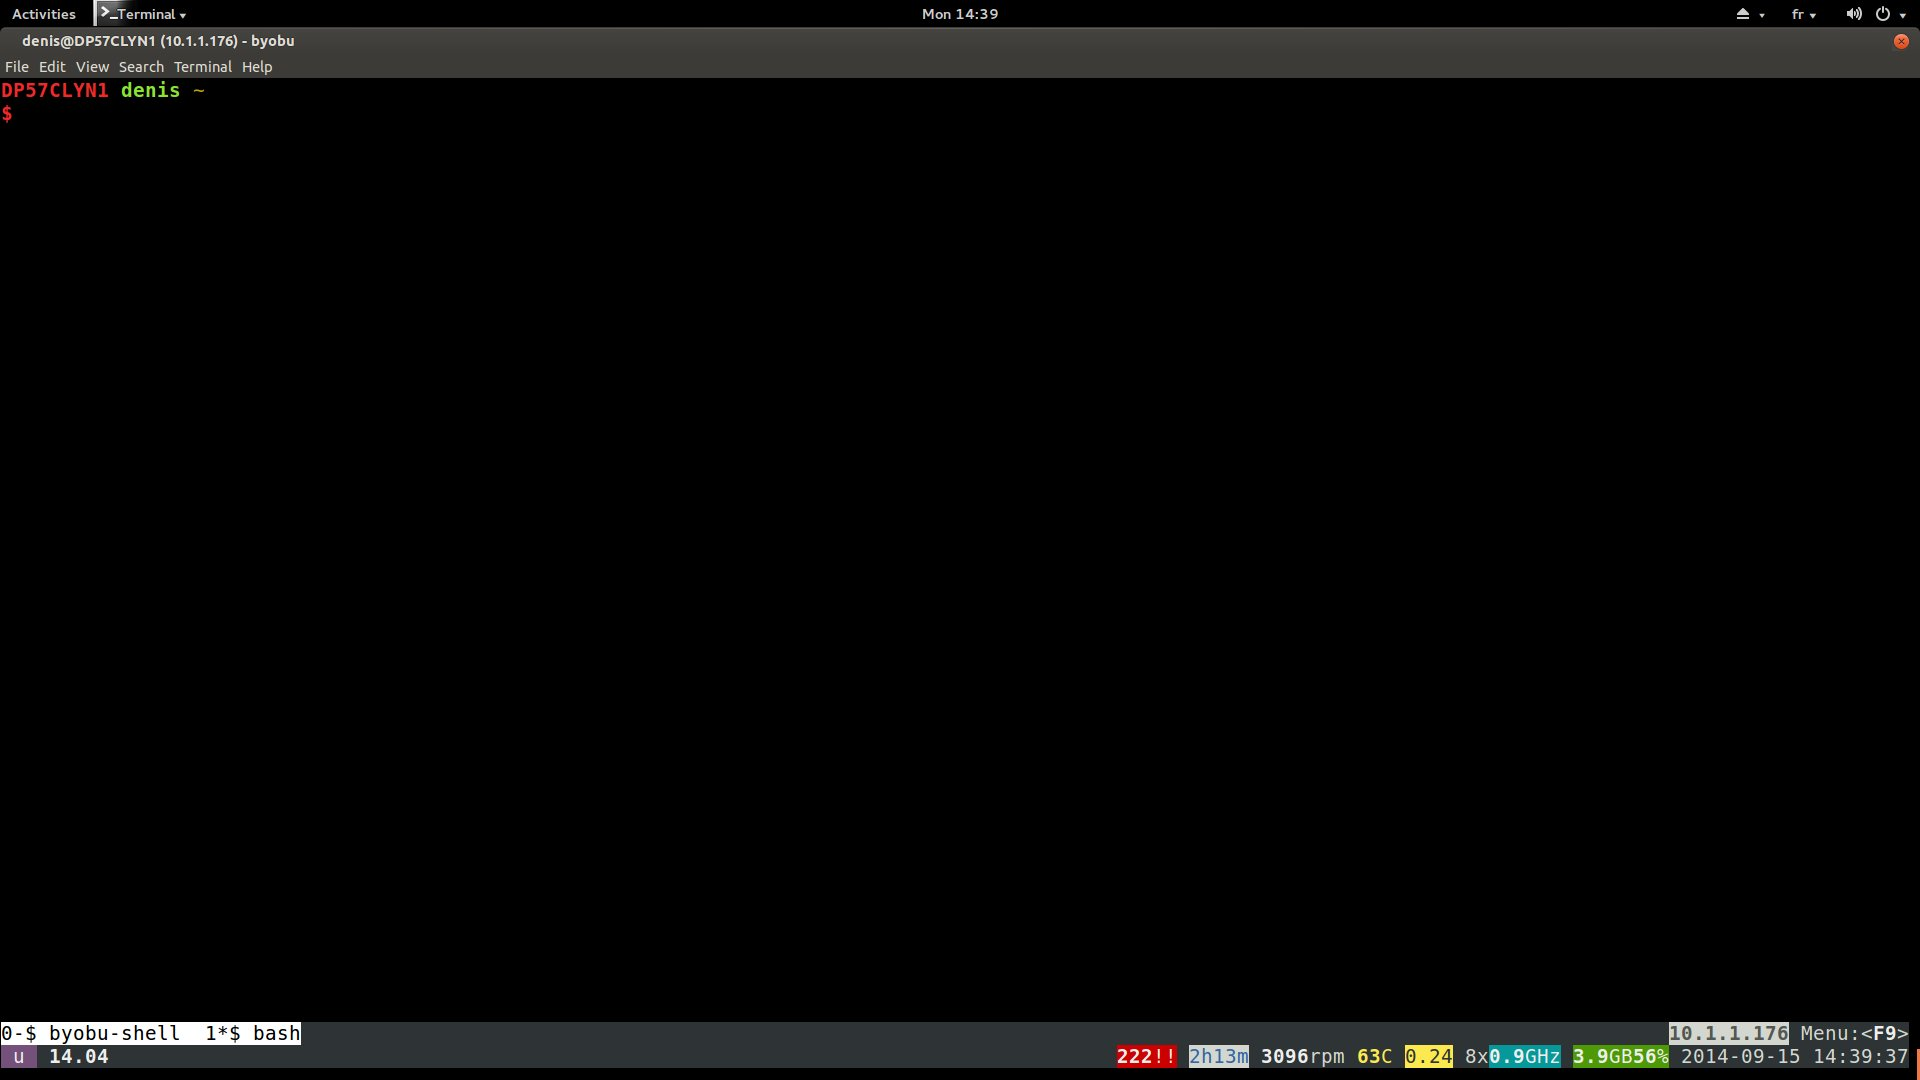
\includegraphics[width=10cm]{boitenoire1}}
    \end{picture}


\end{frame}






%*****************************************************************************************************************************************************


\subsection{Aide sur les commandes}

\begin{frame}[fragile]
    \frametitle{Aide sur les commandes}
    Toutes les commandes unix, sont bien documentées. L'accès à cette documentation se fait à l'aide de la commande \textbf{man} (\textbf{man}ual).
    \tiny    
    \begin{verbatim}
[puthier@mamachine] man tail

TAIL(1)                            Manuel de l utilisateur Linux                                             TAIL(1)

NOM
       tail - Afficher la dernière partie d'un fichier.

SYNOPSIS
       tail  [-c  [+]N[bkm]] [-n [+]N] [-fqv] [--bytes=[+]N[bkm]] [--lines=[+]N] [--follow] [--quiet] [--silent] [--verbose] [--help]
       [--version] [fichier...]
       tail [{-,+}Nbcfklmqv] [fichier...]

DESCRIPTION
       Cette page de manuel documente la version GNU de tail ([NDT] tail = queue).
                          ...
    \end{verbatim}
    \normalsize
\end{frame}



\begin{frame}[fragile]
    
    On trouvera dans l'aide une section ``SYNOPSIS'' --> vue d'ensemble des options du programme. Dans cette section, le principe pour les arguments est le suivant:
    \begin{itemize}
            \item Tout ce qui se trouve entre crochets est facultatif. Ce qui n'est pas entre crochet est nécessaire.
    
            \item Tout ce qui se trouve entre accolade correspond à un choix (souvent exclusif).
    \end{itemize}


    \vspace{0.8mm}
    La rubrique ``OPTIONS'' explique l'influence de chacune des options sur le déroulement du programme. 

\end{frame} 




\begin{frame}[fragile]

  \begin{itemize}
    \item Pour effectuer une recherche dans l'aide on tapera la chaine de caractère recherchée précédée du caractère \textit{/} \\(ex: \textit{/OPTIONS} pour rechercher le terme ``OPTIONS''. 
    \item Pour aller à la prochaine occurrence on utilisera la touche ``n'' (\textbf{n}ext) pour se rendre à l'occurrence précédente on utilisera ``<shift> + n''.
    \item On utilisera ``<ctrl> + <'' et ``<ctrl> + <shift>+<'' pour se rendre à la fin et au début du fichier d'aide respectivement.
    \item On utilisera ``q'' pour quitter l'aide (\textbf{q}uit).
    \end{itemize}

\end{frame}


\begin{frame}[fragile]
    
Recherche de termes à travers les fichiers d'aide.\\

    \vspace{0.8mm}
    On pourra utiliser la commande \textbf{man} avec l'option ``-k''. On recherchera alors l'occurrence d'une chaîne de caractères donnée dans tous les paragraphes ``description'' des fichiers d'aide. On obtiendrait le même résultat avec la commande \textbf{apropos} 
   
 
    \begin{verbatim}
[puthier@mamachine] man -k jpeg
    \end{verbatim}
    \tiny
    \begin{verbatim}
jpeg2ktopam (1)      - convert JPEG-2000 code stream to PAM/PNM
jpeg2yuv (1)         - Convert jpeg images to the yuv format.
jpegicc (1)          - little cms ICC profile applier for JPEG.
jpegtopnm (1)        - convert JPEG/JFIF file to PPM or PGM image
jpegtran (1)         - lossless transformation of JPEG files
lav2wav (1)          - Extract the audio out of MJPEG container files to stdout
lav2yuv (1)          - Convert a MJPEG file to raw yuv
    \end{verbatim}

    \normalsize


\end{frame}


%*****************************************************************************************************************************************************


\section{Fichiers et répertoires}

\frame
{
%\setbeamercolor{block body}{bg=OliveGreen,fg=white}
\begin{block}{}
\begin{center}
\begin{huge}
Fichiers et répertoires
 \end{huge}
\end{center}
\end{block}

}

\subsection{Organisation des fichiers sous Linux}

\begin{frame}[fragile]
    \frametitle{Organisation des fichiers sous Linux}
    \begin{itemize}
    \item les objets (fichiers, répertoires) sont organisés en arborescence.
        \begin{itemize}
        \item chaque objet est désigné par un chemin d'accès.
        \item 2 éléments à connaitre: votre position, la position du fichier/répertoire d'intérêt.
        \end{itemize}
    \end{itemize}
\end{frame}

\begin{frame}[fragile]
\setlength{\unitlength}{1mm}
\begin{picture}(10,10)
\put(35,-15){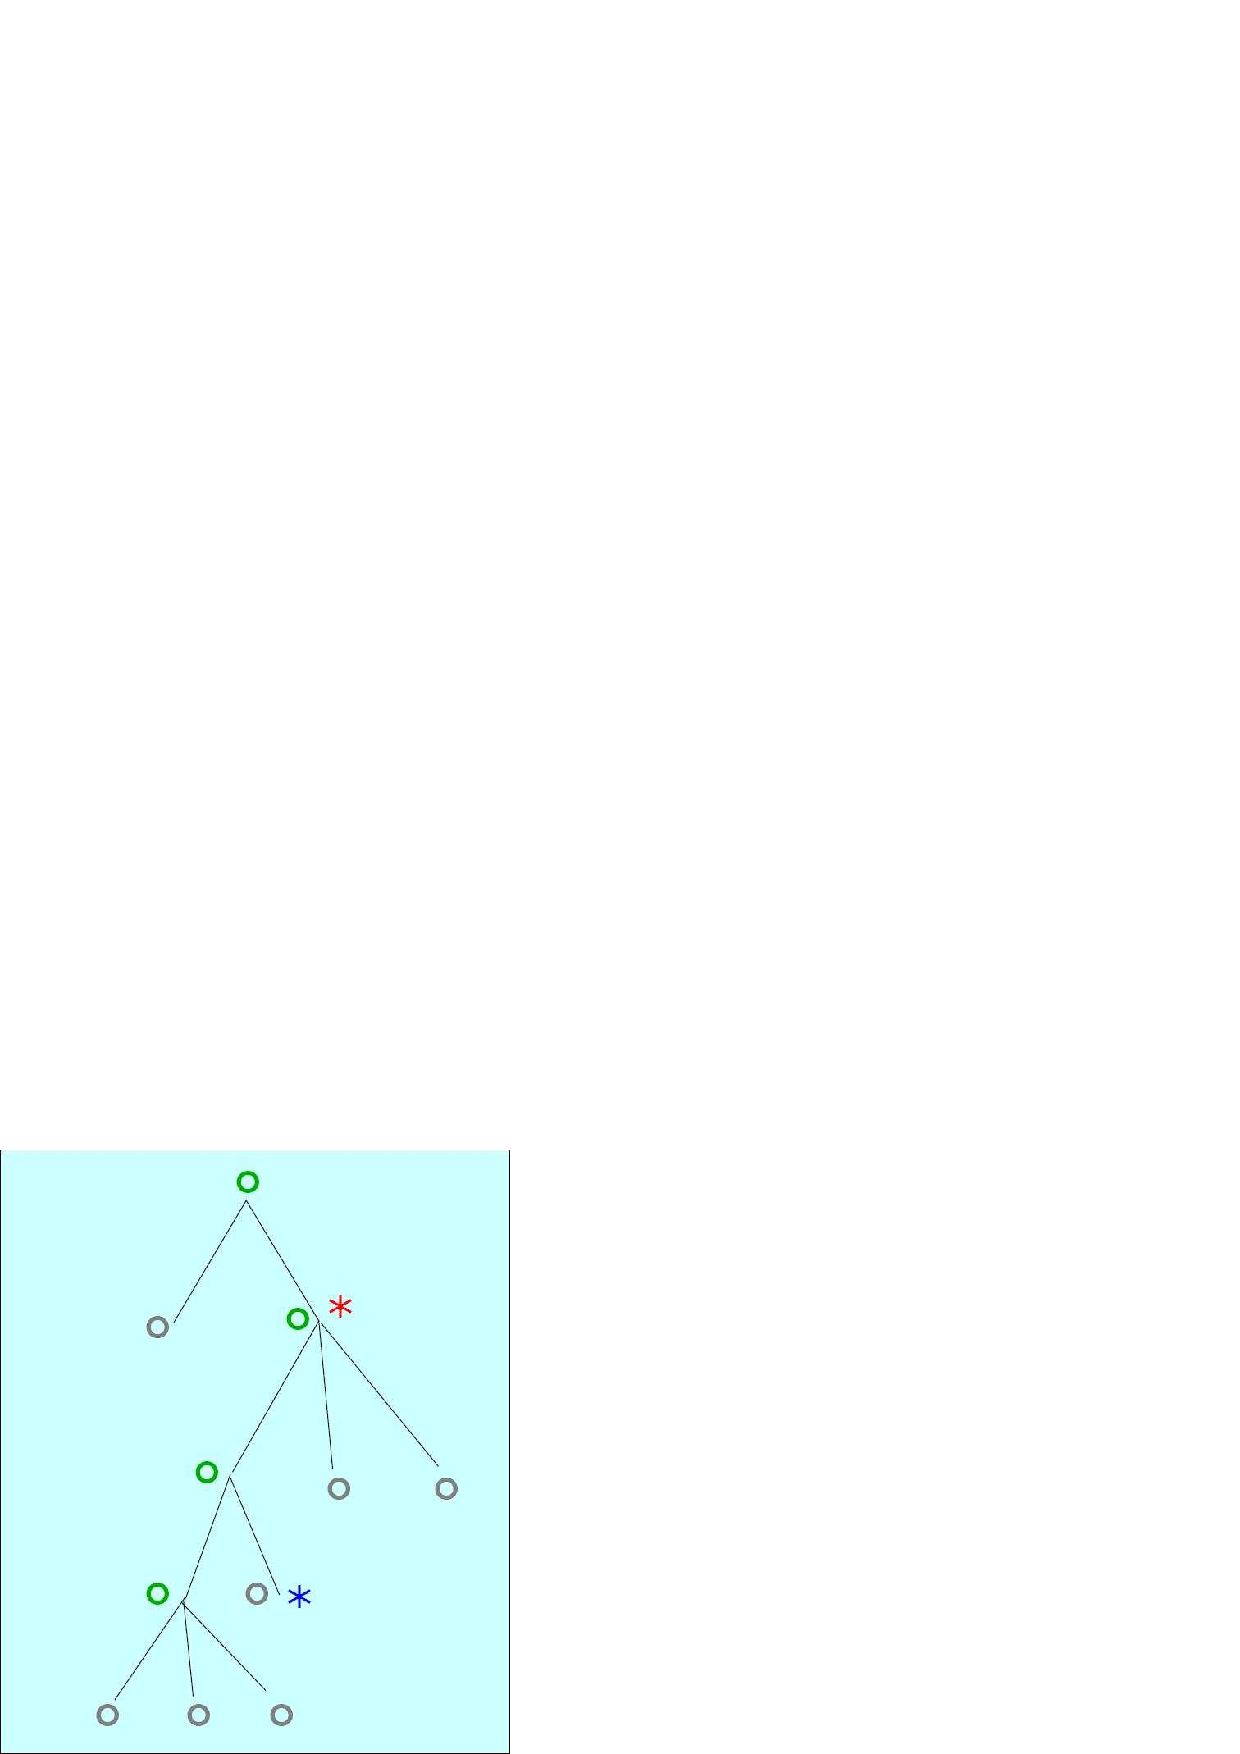
\includegraphics[ width=8cm]{arbo1.pdf}}
  \end{picture}

\end{frame}

\begin{frame}[fragile]
    
        \begin{itemize}
        \item Le repertoire ``racine'' est désigné par ``/''.
            \begin{itemize}
            \item --> $\sim$  C:$\backslash$ sous windows 
            \item contient un certain nombre de sous répertoires (/bin, /boot, ..., /var).
            \end{itemize}
        \end{itemize}

\end{frame}

\begin{frame}[fragile]
	/bin Programmes système (\textbf{bin}aries).\\
    /boot Noyau, Bootmanager.\\
    /dev Fichiers des périphériques (\textbf{dev}ices).\\
    /etc Fichiers de configuration.\\
    /home Répertoires des utilisateurs.\\
    /lib Librairies partagées.\\
    /mnt Répertoire de montage pour cdrom, floppy... (\textbf{m}ou\textbf{nt}).\\
    /opt Installations supplémentaires.\\
    /proc Informations sur le système et les processus en cours (\textbf{proc}ess).\\
    /root Répertoire personnel de \textbf{root}.\\
    /sbin Programmes système pour le root.\\
    /tmp Données \textbf{t}e\textbf{mp}oraires.\\
    /usr Programmes des utilisateurs.\\
    /var Fichiers divers et certains fichiers de logs (\textbf{var}iable)\\

\end{frame}


\begin{frame}[fragile]

    \begin{itemize}
    \item Le répertoire ``home''.
        \begin{itemize}
        \item Contient les dossiers de travail et de configuration de chacun des utilisateurs \\
        /home/puthier, /home/dupont, /home/duchsmock, ...
        \item Il peut être symbolisé par $\sim$:\\
        Si je suis connecté en tant que ``puthier'':\\
         $\sim$ == /home/puthier\\
        Si je suis connecté en tant que ``martin'':\\
         $\sim$ == /home/martin
        \end{itemize}
    \end{itemize}

\end{frame}

\subsection{Chemins relatifs et absolus}

\begin{frame}[fragile]
\frametitle{Chemins relatifs et absolus}

	\begin{itemize}
	 \item Chemin absolu: se réfère à la racine ``/''.
	 \item Chemin relatif: se réfère au répertoire courant.
	 \item Ex: On se trouve dans le répertoire ``Document''. On désigne le fichier ``toto.txt''

	\begin{itemize}
		\item chemin relatif au répertoire ``Document'': toto.txt 
		\item chemin absolu du fichier toto.txt: /home/puthier/Documents/toto.txt
	\end{itemize}
	\end{itemize}

\end{frame}


\begin{frame}[fragile]
  \setlength{\unitlength}{1mm}
  \begin{picture}(20,20)
  \put(35,-15){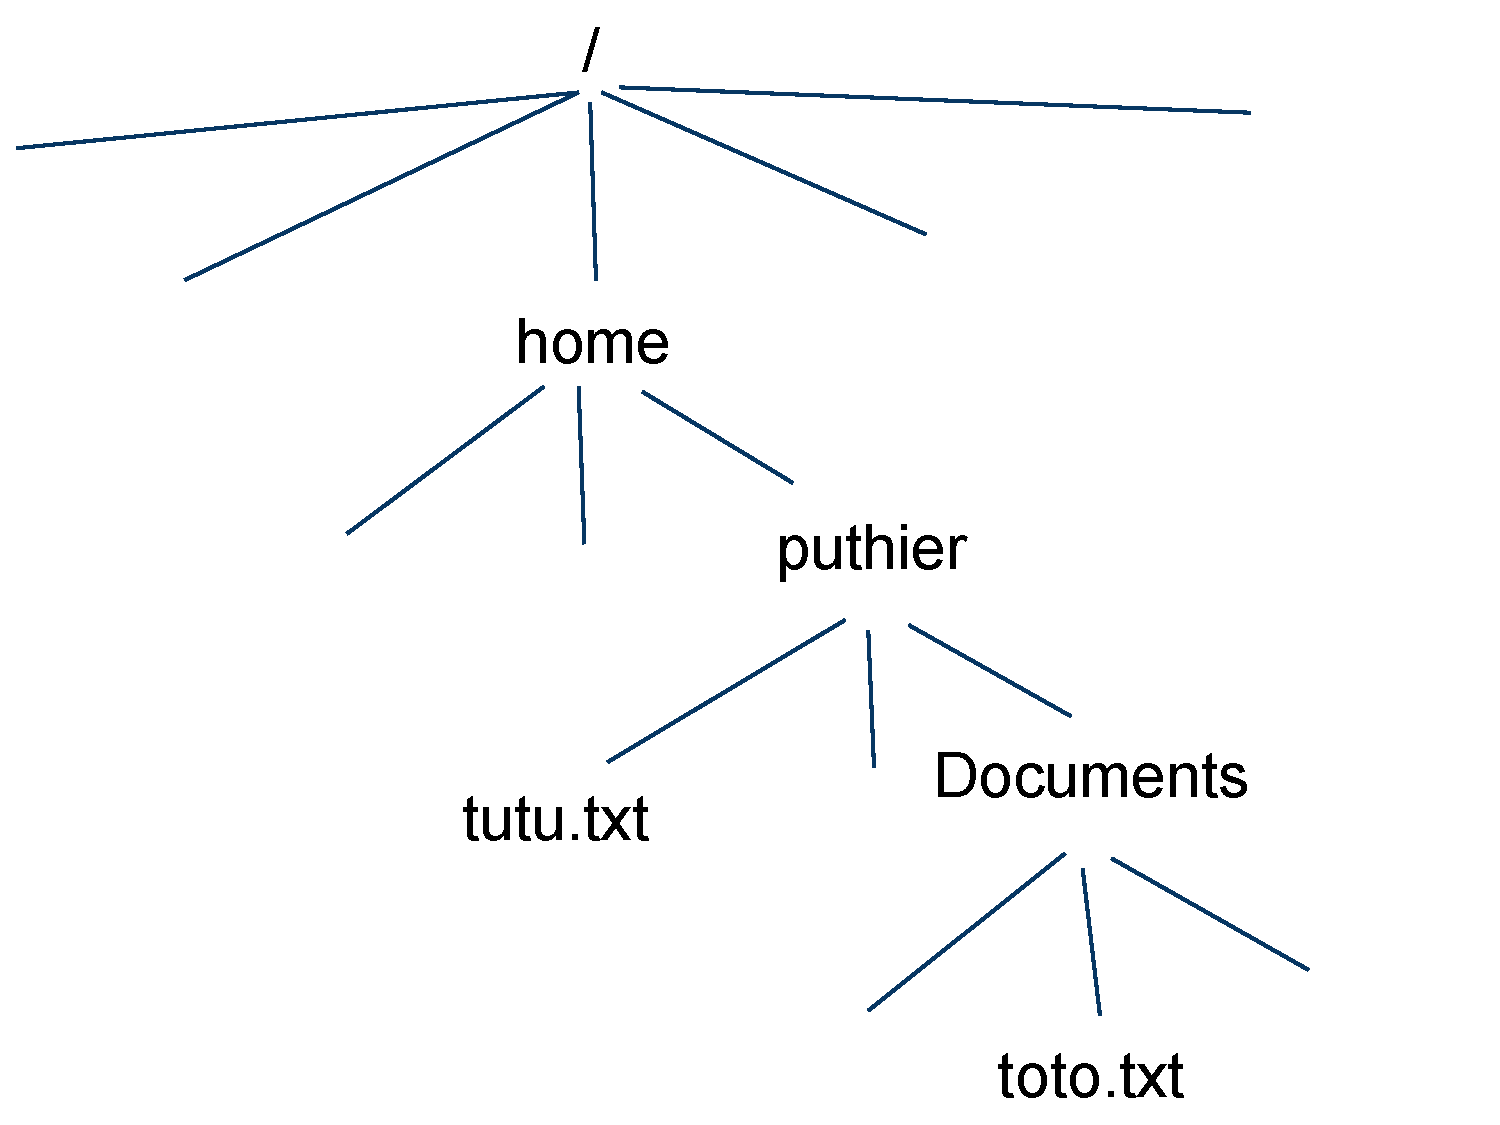
\includegraphics[width=6cm]{arbo2.pdf}}
    \end{picture}
\end{frame}

\begin{frame}[fragile]

        \begin{itemize}
            \item  En écriture relative ``..'' signifie ``répertoire supérieur''
            \item  Ex: On se trouve dans le répertoire ``Document''. On désigne le fichier ``tutu.txt''\\
			\begin{itemize}
              \item chemin relatif au fichier tutu.txt:\\
              ../tutu.txt \\
              \item chemin absolu du fichier tutu.txt: \\
              /home/puthier/tutu.txt\\
        	\end{itemize}
        \end{itemize}
\end{frame}

\begin{frame}[fragile]

        \begin{itemize}
            \item  En ecriture relative ``./'' signifie ``le répertoire courant''
            \item  Ex: On se trouve dans le répertoire ``Document''.\\
              ./toto.txt <=> toto.txt \\
        \end{itemize}

\end{frame}

\subsection{Opérations sur les dossiers}

\begin{frame}[fragile]
    \frametitle{Opérations sur les dossiers}
        \begin{itemize}
            \item  La commande ``cd'' (\textbf{c}hange \textbf{d}irectory)
            \item  Ex 1: On se trouve dans Document. On souhaite se rendre dans ``/home/puthier''\\
			\begin{itemize}
				\item En absolue: \\

              \begin{verbatim} cd /home/puthier \end{verbatim}
              ou 
              \begin{verbatim} cd ~ \end{verbatim}
              \item En relatif: \\
              \begin{verbatim} cd .. \end{verbatim}
        \end{itemize}
        \end{itemize}
\end{frame}

\begin{frame}[fragile]
        \begin{itemize}

            \item  Ex 2: On se trouve dans ``Document''. On souhaite se rendre à la racine\\
        \begin{itemize}
	              \item En absolue: \\
              \begin{verbatim} cd / \end{verbatim}
              \item En relatif: \\
              \begin{verbatim} cd ../../.. \end{verbatim}
        \end{itemize}
            \item \textbf{NB}: Pensez toujours à utiliser la \\``complétion'' (touche tabulation)
        \end{itemize}

\end{frame}



\begin{frame}[fragile]
        \begin{itemize}
  
              \item \textbf{pwd}, \textbf{p}rint \textbf{w}orking \textbf{d}irectory (afficher le répertoire courant)\\
              Ex: on se trouve dans ``Document''\\

          \begin{verbatim}
[puthier@mamachine] pwd
 /home/puthier/Documents
          \end{verbatim}

            \item \textbf{ls}, \textbf{l}i\textbf{s}t (lister les fichiers et dossiers d'un répertoire)\\
            Ex: on se trouve dans ``Document''\\
            \vspace{0.8mm}
          \begin{verbatim}
[puthier@mamachine] ls 
 toto.txt
[puthier@mamachine] ls  /home/puthier
 tutu.txt
[puthier@mamachine] ls  ~
 tutu.txt
          \end{verbatim}
        \end{itemize}

\end{frame}

\begin{frame}[fragile]

        \begin{itemize}

            \item Les options de \textbf{ls}\\
			\begin{itemize}
             \item ls -l: (\textbf{l}ong) affiche les droits, les tailles et les dates de création/modification des fichiers et répertoires \\
             \item ls -a: (\textbf{a}ll) affiche tous les fichiers et répertoires, même les fichiers/dossiers cachés (leurs noms commencent par ``.'')  \\
             \item ls -R: (\textbf{r}ecursive) affiche tous les fichiers et le contenu des dossiers.\\

	         \item ls --sort=time: trie les fichiers par date de création\\
             \item ls --sort=size: trie les fichiers par tailles\\

             \item ls -1: présente les nom des fichiers/dossiers en une seule colonne\\
			\end{itemize}
            \item On peut combiner les options des commmandes:\\
            \begin{verbatim}[puthier@mamachine] ls -la /home/puthier/\end{verbatim}
        \end{itemize}

\end{frame}

\begin{frame}[fragile]
        \begin{itemize}

            \item \textbf{mkdir}, \textbf{m}a\textbf{k}e \textbf{d}irectory (créer un répertoire)\\
            Ex: on se trouve dans ``Document''\\

         \begin{verbatim}
    [puthier@mamachine] mkdir analyses
    [puthier@mamachine] ls
     analyses tutu.txt
          \end{verbatim}

            \item \textbf{rmdir}, \textbf{r}e\textbf{m}ove \textbf{d}irectory (déléter un répertoire)\\
            Ex: on se trouve dans ``Document''\\
            \vspace{0.8mm}
          \begin{verbatim}
    [puthier@mamachine] rmdir analyses
    [puthier@mamachine] ls
     tutu.txt
          \end{verbatim}

            \item \textbf{rmdir} équivaut à ``rm -Rf analyses''. NE PAS UTILISER CETTE COMMANDE !!!!
        \end{itemize}

\end{frame}



\begin{frame}[fragile]

\textbf{NB}: Les caractères ``\textbf{joker}''. Permettent de désigner un ensemble de fichiers 
      
      \begin{itemize}
              \item ''$?$`` : Désigne un caractére quelconque (présent).
              \item ''*``: Désigne un ensemble de caractères quelconques (présents ou absents). 
          \begin{verbatim}
[puthier@mamachine] ls 
 file12.txt  file1.txt  file2.txt  file.txt f.sh

[puthier@mamachine] ls file*
 file12.txt  file1.txt  file2.txt  file.txt

[puthier@mamachine] ls file?.txt
 file1.txt  file2.txt

          \end{verbatim}
        \end{itemize}

\end{frame}


\begin{frame}[fragile]
        \begin{itemize}


           \item \textbf{du} (\textbf{d}isk usage) afficher la taille totale des fichiers contenus dans un répertoire:\\
           \begin{verbatim}
[puthier@mamachine] du -sh /home/puthier/
 824M    /home/puthier/
           \end{verbatim}

            \item Options:\\
            du -h: (\textbf{h}uman readable) (affiche la taille en ko, Mo, Go)\\

            du -s: (\textbf{s}um) (affiche le somme de tous les fichiers et sous répertoires)

        \end{itemize}

\end{frame}


\subsection{Opérations sur les fichiers}

\begin{frame}[fragile]

\frametitle{Opérations sur les fichiers}

        \begin{itemize}

           \item \textbf{cat}: afficher le contenu d'un fichier:
          \begin{verbatim}
[puthier@mamachine] cat /home/puthier/tutu.txt
          \end{verbatim}

           \item \textbf{less/more}: afficher le contenu d'un fichier page par page:
          \begin{verbatim}
[puthier@mamachine] less /home/puthier/tutu.txt
          \end{verbatim}
            On utilisera ``<ctrl> + <'' et ``<ctrl> + <shift>+<'' pour se rendre à la fin et au début du fichier d'aide respectivement.
            On utilisera ``q'' pour quitter l'aide (\textbf{q}uit).
          \begin{verbatim}
[puthier@mamachine] more /home/puthier/tutu.txt
          \end{verbatim}

        \end{itemize}

\end{frame}


\begin{frame}[fragile]
\frametitle{Opérations sur les fichiers}

\begin{itemize}

\item \textbf{NB}: Sous Unix et windows le retour à la ligne est codé différemment dans les fichiers:
\end{itemize}
         
\begin{verbatim}
[puthier@mamachine] od -c exemple.unix.txt
0000000   A  \n   B  \n   C  \n
0000006

[puthier@mamachine] od -c exemple.win.txt 
0000000   A  \r  \n   B  \r  \n   C  \r  \n 
0000012
\end{verbatim}

\end{frame}



\begin{frame}[fragile]


        \begin{itemize}

           \item Connaître les droits des fichiers, leurs tailles ...:\\
          \begin{verbatim}
[puthier@mamachine] ls -l /home/puthier/
          \end{verbatim}
        \end{itemize}
\end{frame}




%% \begin{frame}[fragile]
%% \setlength{\unitlength}{1mm}
%% \begin{picture}(20,20)
%% \put(0,-10){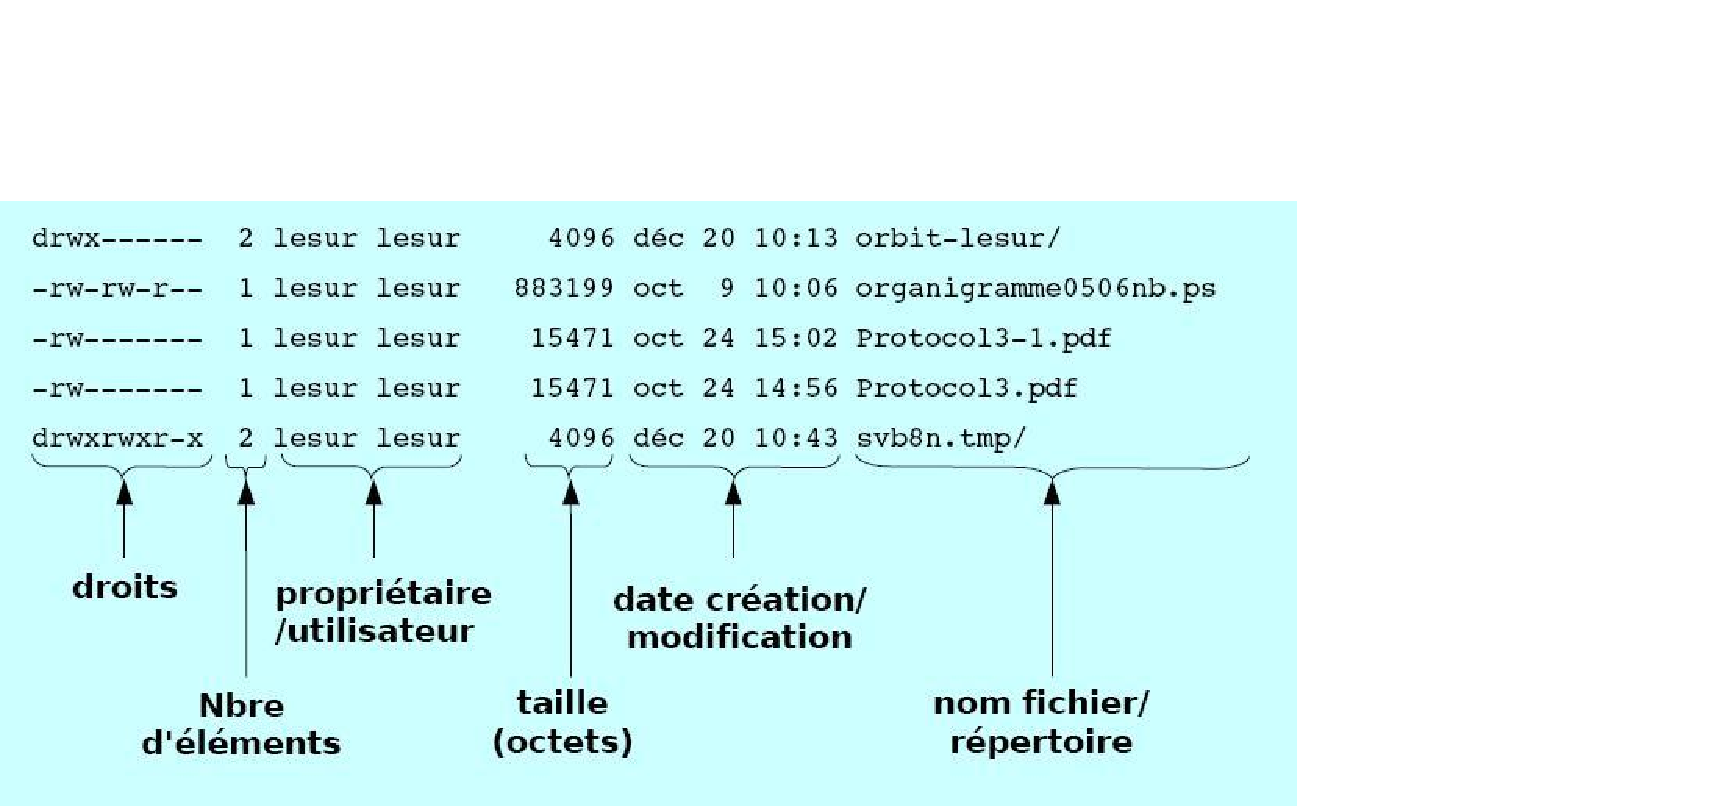
\includegraphics[ width=9cm]{arbo8.pdf}}
%%   \end{picture}

%% \end{frame}


\begin{frame}[fragile]

\begin{flushleft}


    \begin{itemize}
      \item chmod, (\textbf{ch}ange \textbf{mod}e) changer\\
           les droits d'un fichier:\\
\begin{small}
    \begin{verbatim}
chmod [ugoa] {+,-,=} [rwx] <Fichier> 
    \end{verbatim}
\end{small}
      \item \textbf{u}ser, \textbf{g}roup, \textbf{o}ther, \textbf{a}ll
      \item \textbf{r}ead, \textbf{w}rite, e\textbf{x}ecute
    \end{itemize}
\setlength{\unitlength}{1mm}
\begin{picture}(20,20)
\put(40,-10){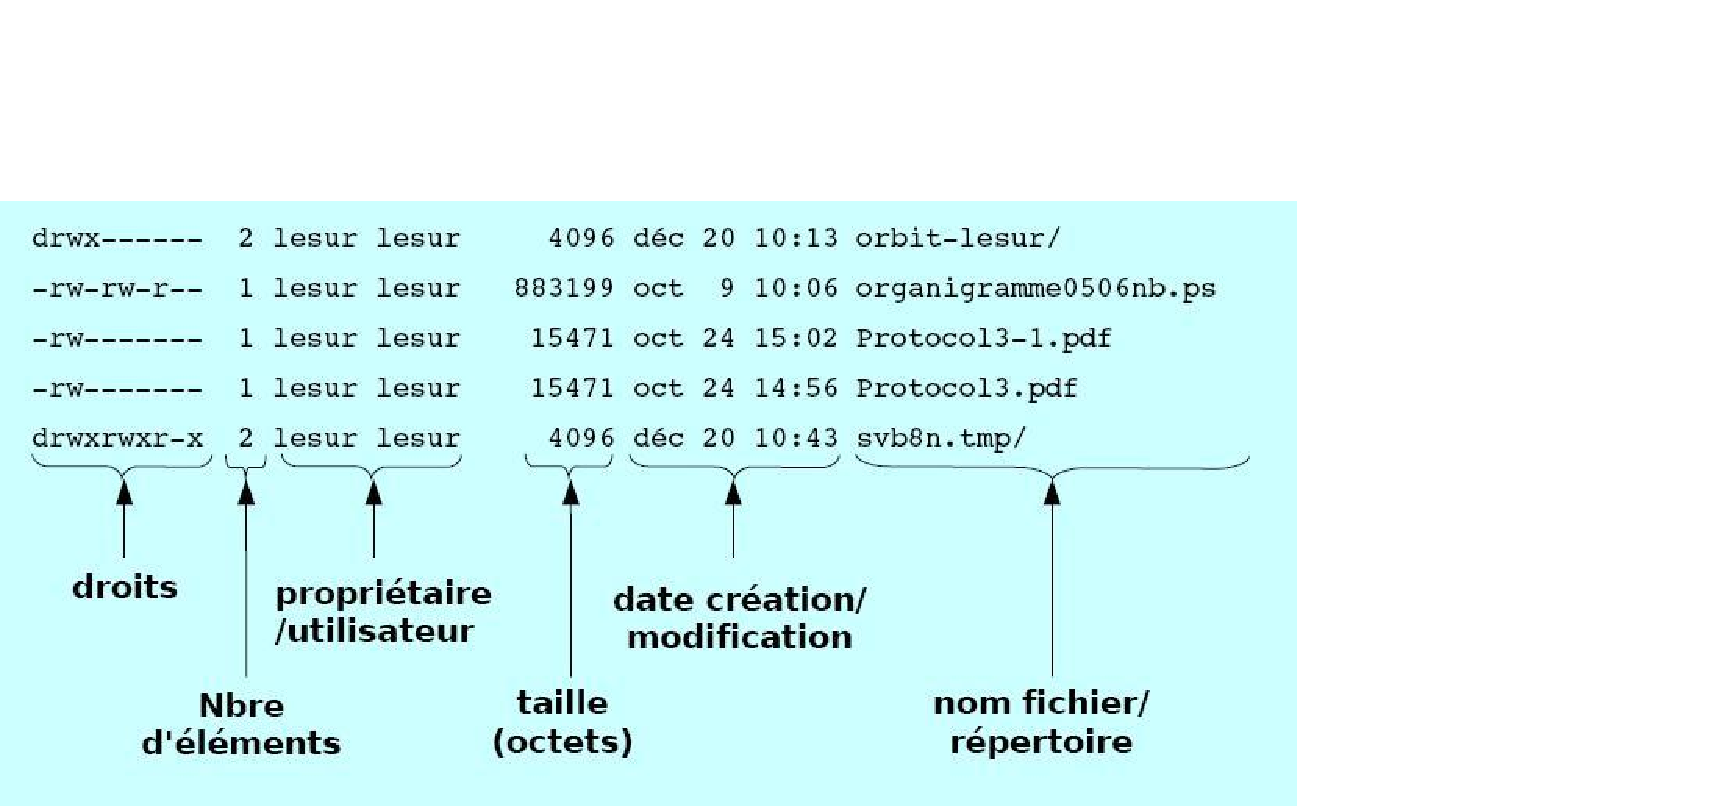
\includegraphics[height=4cm]{arbo8.pdf}}
      \end{picture}

\end{flushleft}

\end{frame}


\begin{frame}[fragile]

    \begin{itemize}

    \item Ex: fichier week.html\\
    \begin{verbatim}
--> -rw-r--r-- 1 puthier users  16K week.html
    \end{verbatim}

    \item Enlever les droits de lecture sur le fichier week.html pour tous sauf l'utilisateur et le groupe:\\
    \begin{verbatim}
[puthier@mamachine] chmod o-r week.html
-rw-r----- 1 puthier users 16K week.html
    \end{verbatim}

    \item Ajouter les droits de lecture/écriture pour tous:
    \begin{verbatim}
[puthier@mamachine] chmod a+rw week.html
-rw-rw-rw- 1 puthier users 16K week.html
    \end{verbatim}

    \end{itemize}

\end{frame}



\begin{frame}[fragile]

    \begin{itemize}

          \item la commande \textbf{wc} (\textbf{w}ord \textbf{c}ount) affiche 3 valeurs:\\
            le nombre de lignes\\
            le nombre de mots (séparés par des blancs)\\
            le nombre d'octets\\
    
        \begin{verbatim}
[puthier@mamachine] wc GSE7671_family.soft
 7899  60663 461473 GSE7671_family.soft
        \end{verbatim}
    
          \item connaître le nombre de lignes dans un fichier:
    
        \begin{verbatim}
[puthier@mamachine] wc -l GSE7671_family.soft
 7889
        \end{verbatim}

    \end{itemize}

\end{frame}

\begin{frame}[fragile]

    \begin{itemize}

          \item la commande \textbf{tail}. Affiche les n dernières lignes d'un fichier.
              \begin{flushleft} 
              \begin{verbatim}
[puthier@mamachine] tail -4 GSE7671_family.soft
 376     -1.02    15393   
 377     NULL    NULL    
 378     NULL    NULL    
 379     0.008     1111    
              \end{verbatim}
              \end{flushleft} 
          \item la commande \textbf{head}. Affiche les n premières lignes d'un fichier.
              \begin{flushleft} 
             \begin{verbatim}
[puthier@mamachine] head -4 GSE7671_family.soft
 ^DATABASE 
 !Database_name 
 !Database_institute 
 !Database_web_link
              \end{verbatim}
              \end{flushleft} 
    \end{itemize}

\end{frame}


\begin{frame}[fragile]

    \begin{itemize}
        \item Copier un fichier:
             \begin{verbatim}
    cp <origine> <destination>
             \end{verbatim}
        \item Exemple (le fichier garde le nom toto.txt):
             \begin{verbatim}
    cp toto.txt ..
             \end{verbatim}

        \item Exemple (copie avec changement de nom):
             \begin{verbatim}
    cp toto.txt ../titi.txt
             \end{verbatim}
\setlength{\unitlength}{1mm}
\begin{picture}(20,20)
\put(68,10){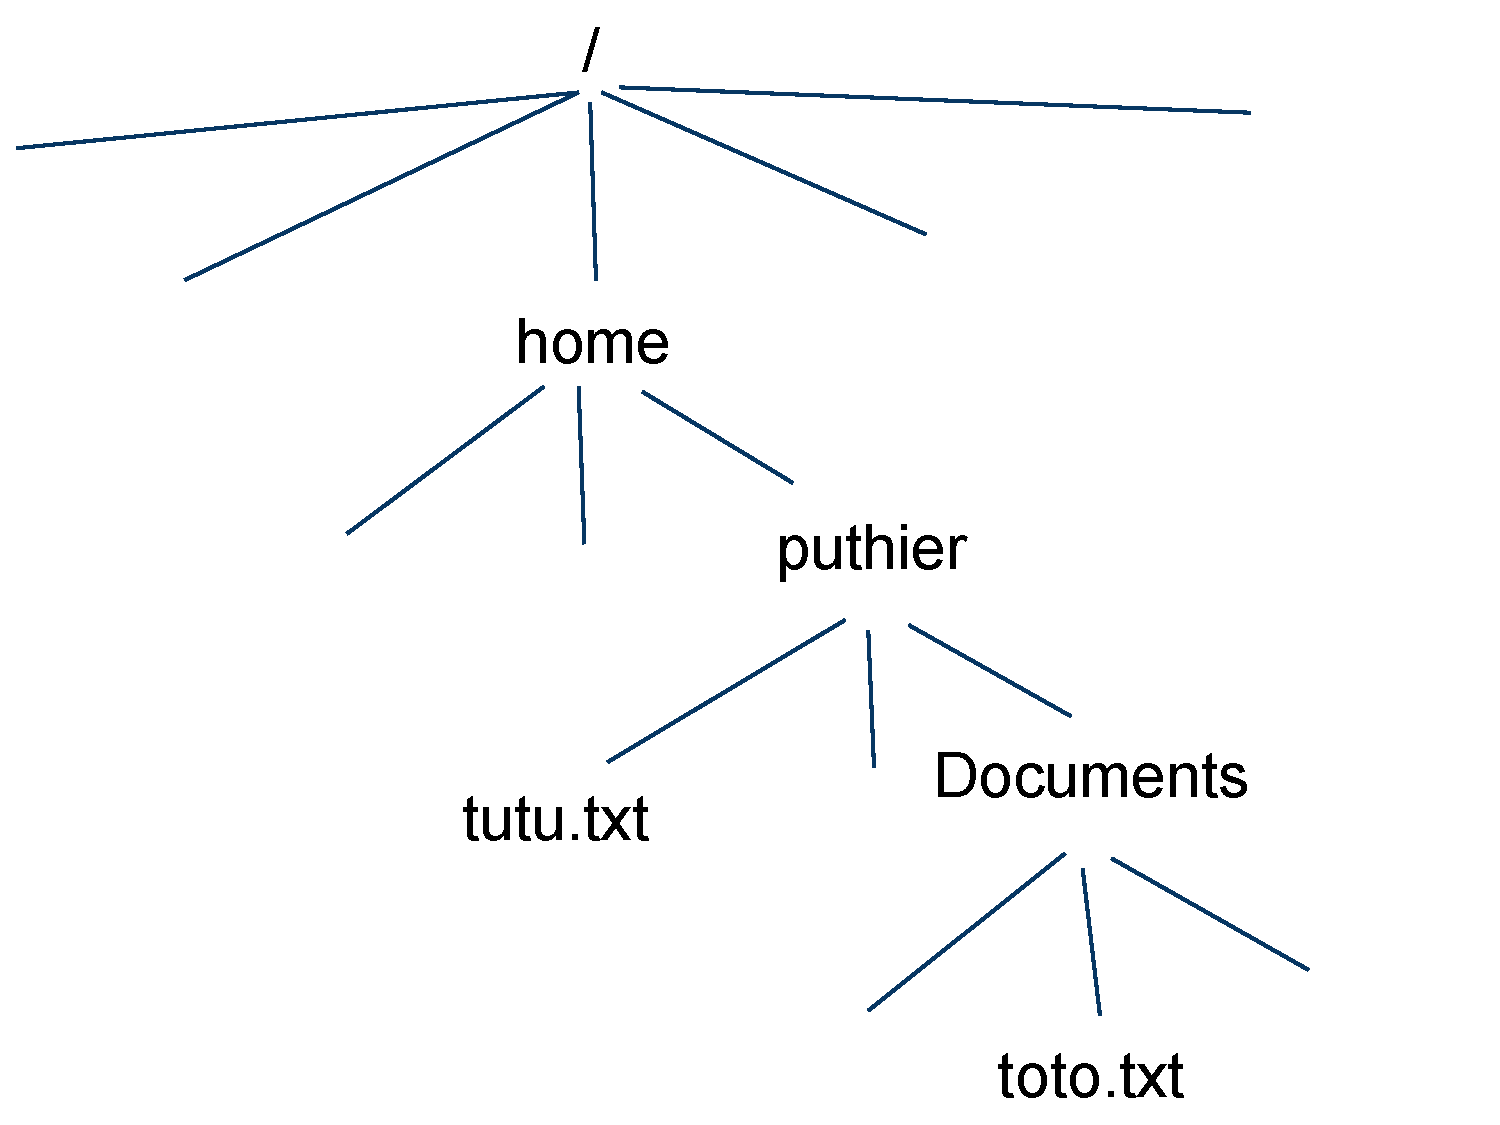
\includegraphics[width=4cm,height=3cm]{arbo2.pdf}}
  \end{picture}

    \end{itemize}
\end{frame}



\begin{frame}[fragile]

    \begin{itemize}
        \item \textbf{mv}: (\textbf{m}o\textbf{v}e), déplacer un fichier:
             \begin{verbatim}
mv <origine> <destination>
             \end{verbatim}
        \item Exemple (le fichier est déplacé et conserve son nom original):
             \begin{verbatim}
mv /home/puthier/Documents/toto.txt /tmp
             \end{verbatim}
        \item Exemple (le fichier est deplacé et renommé):
             \begin{verbatim}
mv /home/puthier/Documents/toto.txt /tmp/f.txt
             \end{verbatim}
        \item \textbf{mv} est utilisé pour renommer les fichiers
             \begin{verbatim}
mv file.old.txt file.new.txt
             \end{verbatim}
    \end{itemize}

\end{frame}


\begin{frame}[fragile]

La fonction \textbf{cut}:

    \begin{itemize}
        \item Pour les fichiers contenant plusieurs colonnes, il est utile de pouvoir
extraire certaines d'entre elles.
             \begin{verbatim}
cut [-fd] <fichier>
             \end{verbatim}
        \item -\textbf{f}=\textbf{f}ield, -\textbf{d}=separator.
        \item Exemple:
             \begin{verbatim}
[puthier@mamachine] cut -f3,5 fichier.txt
             \end{verbatim}
 Extrait la 3ième et la 5ième colonnes du fichier ``fichier.txt''. Par défaut, le séparateur de colonne est une tabulation. 
    \end{itemize}

\end{frame}

\section{Redirection}

\frame
{
%\setbeamercolor{block body}{bg=OliveGreen,fg=white}
\begin{block}{}
\begin{center}
\begin{huge}
Redirection
 \end{huge}
\end{center}
\end{block}

}


\subsection{Entrées-Sorties (E$\backslash$S) d'un processus.}

\begin{frame}[fragile]
\frametitle{Entrées-Sorties (E$\backslash$S) d'un processus.}
  \begin{small}
Dans un processus les flux E$\backslash$S sont au nombre de trois.
                  \begin{itemize}
                        \item L'\textbf{entrée standard} est le flux d'entrée par lequel du texte ou toute autre donnée peut être entré dans un programme.
                        \item La \textbf{sortie standard} est le flux de sortie dans lequel les données sont écrites par le programme. Les données sont habituellement écrites à l'écran.
                        \item L'\textbf{erreur standard} est le flux de sortie permettant aux programmes d'émettre des messages d'erreur et des diagnostics.
                \end{itemize}
  \end{small}
\setlength{\unitlength}{1mm}
\begin{picture}(20,20)
\put(10,2){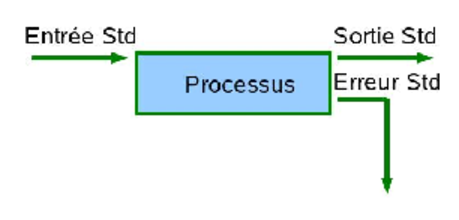
\includegraphics[height=1.8cm]{proc1.pdf}}
      \end{picture}

\end{frame}


\subsection{Les opérateurs de redirection}

\begin{frame}[fragile]
\frametitle{Les opérateurs de redirection}
            \begin{itemize}
          \item On utilise des opérateurs pour rediriger un fichier vers l'entrée d'un processus ou rediriger les sorties d'un processus.
                  \begin{itemize}
                        \item ''$<$`` Suivi du nom du fichier indique sa redirection vers un processus donné.
                        \item ''$>$``: redirection de la sortie standard d'un processus vers un fichier (celui-ci est écrasé).
                        \item ''$>>$``: redirection de la sortie standard d'un processus vers un fichier (ajout)
                        \item ''$2>$``: redirection de l'erreur standard vers un fichier.
                \end{itemize}
      \end{itemize}
\end{frame}

\begin{frame}[fragile]
            \begin{itemize}
          \item Exemple 1: les noms des fichiers présents dans ``/tmp'' sont stockés dans le fichier ``tmp.txt''
             \begin{verbatim}
[puthier@mamachine] ls /tmp > tmp.txt
             \end{verbatim}
          \item Exemple 2: On ajoute la liste des fichiers du dossier ``/home/puthier''
             \begin{verbatim}
[puthier@mamachine] ls /home/puthier >> tmp.txt
             \end{verbatim}
          \item Exemple 3: On concatène des fichiers. 
\begin{small}
             \begin{verbatim}
[puthier@mamachine]  echo "123" > f1.txt
[puthier@mamachine]  echo "456" > f2.txt
[puthier@mamachine]  cat f*.txt >> result.txt
[puthier@mamachine]  cat result.txt
123
456
            \end{verbatim}          
\end{small}
      \end{itemize}
\end{frame}


\subsection{Les tubes (pipes).}

\begin{frame}[fragile]
\frametitle{Les tubes (pipes)}
    \begin{itemize}
        \item Les processus générés par les commandes peuvent s'enchaîner.
        \item Un tel enchainement est symbolisé ``par le caractère ''|`` (tube ou ''pipe``).
    \end{itemize}
\setlength{\unitlength}{1mm}
\begin{picture}(20,20)
\put(0,-15){\includegraphics[height=2.5cm]{filtre.pdf}}
      \end{picture}


\end{frame}

\begin{frame}[fragile]

Exemple d'enchaînement:
\begin{small}
             \begin{verbatim}
[puthier@mamachine] cat file_test.txt
 Martine
 Alain
 Julien
 Aline
 Aline
 Robert

[puthier@mamachine] cat file_test.txt | sort | uniq
 Alain
 Aline
 Julien
 Martine
 Robert
     \end{verbatim}
\end{small}

\end{frame}


\begin{frame}[fragile]

\begin{itemize}
\item Exemple d'enchaînement:
\end{itemize}

\begin{verbatim}
[puthier@mamachine]  cat test.txt
Martine
Alain
Julien
Aline
Aline
Robert

[puthier@mamachine] grep -E "^[AM].*e$" test.txt | head -2
Martine
Aline
\end{verbatim}

\end{frame}


\section{Expressions régulières}

\frame
{
%\setbeamercolor{block body}{bg=OliveGreen,fg=white}
\begin{block}{}
\begin{center}
\begin{huge}
Expressions régulières
 \end{huge}
\end{center}
\end{block}

}


\subsection{Définition}


\begin{frame}[fragile]
\frametitle{Définition}

    \begin{itemize}
        \item Elles permettent de décrire une motif au sein d'une chaîne de caractères. \\
    \end{itemize}
\begin{small}
\begin{tabular}{|r|l|}
\hline
         . & un caractère quelconque.\\
         $[a-z]$ & une lettre minuscule (interval, ex: $[u-w]$). \\
         $[A-Z]$ & une lettre majuscule (interval, ex: $[A-E]$). \\
         $[ABc]$  & A ou B ou c.\\
         $[$\^{}$ABab]$ & Toute lettre différente de a et b.\\
         \^{} & Début de ligne.\\
         \$ & Fin de ligne.\\
         x* & 0 ou n fois le caractères $x$.\\
         x+ & 1 ou n fois le caractère $x$.\\
         x\{n,m\} & Le caractère $x$ répété entre n et m fois.\\
         $\backslash$ & Caractère d'échappement.\\
\hline
\end{tabular}
\end{small}
\end{frame}


\begin{frame}[fragile]

    \begin{itemize}
        \item Exemples\\
        \vspace*{2mm}
        \begin{tabular}{|r|l|}
        \hline
                  $\backslash$.txt\$ & Toute chaîne finissant par ``.txt''\\
                  \^{}$[A-B]$ & Une chaîne débutant par une majuscule.\\
                  \^{}.\{4,6\}$\backslash$.txt\$ & Quatre à 6 caractères suivis de ``.txt``\\
                  \^{}$[A-Z]$.*$\backslash$.txt\$  & Une chaîne débutant par une majuscule\\ & et finissant par ''.txt``\\
                  \^{}\$ & Une chaîne de caractères vide.\\
                  \^{}$[$\^{}$0-9]$*$\backslash$.sh\$ & Une chaîne ne contenant pas de chiffres\\ & et se terminant par ''.sh``\\

        \hline
        \end{tabular}

    \end{itemize}

\end{frame}




\section{Les filtres}

\frame
{
%\setbeamercolor{block body}{bg=OliveGreen,fg=white}
\begin{block}{}
\begin{center}
\begin{huge}
Les filtres
 \end{huge}
\end{center}
\end{block}

}

\subsection{Définition}


\begin{frame}[fragile]
\frametitle{Définition}
\begin{itemize}
  \item Un filtre est une commande capable de lire un flux sur son entrée standard, d'effectuer un traitement et d'écrire le résultat sur sa sortie standard. On peut les enchaîner avec des ``tubes''.
 
\item Exemple de filtres:
            \begin{itemize}
             \item  \textbf{grep}, \textbf{sort}, \textbf{tr}, \textbf{sed}, \textbf{wc}, \textbf{head},\\ \textbf{tail}, \textbf{paste}, \textbf{awk}, \textbf{(perl)}, ...
            \end{itemize}

\end{itemize}

\end{frame}
 
\subsection{La commande grep}

\begin{frame}[fragile]

\frametitle{La commande grep}

    La commande \textbf{grep}: (\textbf{g}eneral \textbf{r}egular \textbf{e}xpression \textbf{p}rocessor) permet de filtrer l'entrée via l'utilisation d'une expression regulière. Son entrée peut être un fichier ou un flux.


    
        \begin{itemize}
            \item L'option \textbf{-E} permet l'utilisation d'expressions réguliéres étendues (ERE).
            \item L'option \textbf{-E} permet l'utilisation d'expressions réguliéres compatibles avec Perl (PCRE).
            \begin{verbatim}
[puthier@mamachine] echo -e "456\n567\n775" |grep -P "^.5"
456
            \end{verbatim}
        \end{itemize}


\end{frame}

\begin{frame}[fragile]

La commande \textbf{grep} (suite).

     \begin{itemize}
        \item A noter l'option \textbf{-r} (\textbf{r}ecursive), permet de rechercher un terme en mode récursif.
        \begin{verbatim}
[puthier@mamachine]  grep -r "toto" ./*
        \end{verbatim}
        \item A noter l'argument -v--invert-match (affiche les lignes ne contenant pas le motif).
        \begin{verbatim}
[puthier@mamachine]  echo -e "123\n456"|grep -v "^1"
456
        \end{verbatim}
    \end{itemize}

\end{frame}


\subsection{La commande sort}
\begin{frame}[fragile]
\frametitle{La commande sort}
    \begin{itemize}
        \item La commande \textbf{sort} (tri).

             \begin{verbatim}
sort [-t  separateur] [-kPOS1[,POS2]] [-nr] <fichier>
             \end{verbatim}

        \item \textbf{n}umérique, \textbf{r}everse. Exemple: tri sur la troisième colonne


             \begin{verbatim}
[puthier@mamachine]  cat toto.txt
        b       1       C
        a       2       B
        c       5       A

[puthier@mamachine]  sort -k3 toto.txt
        c       5       A
        a       2       B
        b       1       C
             \end{verbatim}
    \end{itemize}

\end{frame}

\subsection{La commande tr}

\begin{frame}[fragile]

\frametitle{La commande tr}

Transpose ou élimine des caractères (\textbf{tr}anslate).
            \begin{verbatim}
   tr [options] chaîne1 chaîne2 <entree >sortie
             \end{verbatim}

    \begin{itemize}
    \item Exemple 1: transposition.
             \begin{verbatim}
[puthier@mamachine]  echo "ABCDE"|tr  'A' 'C'
 CBCDE

[puthier@mamachine]
 tr 'url' 'URL'  < week.html > result.txt

[puthier@mamachine] echo "ABCDE"|tr -d 'A'
 BCDE
             \end{verbatim}
    \end{itemize}

\end{frame}

 \subsection{La commande sed}

\begin{frame}[fragile]
 \frametitle{La commande sed}
  La commande \textbf{sed}: "\textbf{s}tream \textbf{ed}itor". etant donné un flux, recherche l'occurence d'une expression réguliére et effectue les modifications. 

    \begin{itemize}
    \item Exemple 
\end{itemize}

             \begin{verbatim}
[puthier@mamachine] echo -e "ABCD\nDEF"
ABCDEF
DEFAA

[puthier@mamachine]  echo -e 'ABCA\nAEA' | sed 's/A/G/'
GBCA
GEA
[puthier@mamachine]  echo -e 'ABCA\nAEA' | sed 's/A/G/g'
GBCG
GEG
             \end{verbatim}
\end{frame}


\section{La commande AWK}

\begin{frame}[fragile]
  \frametitle{La commande awk}

  \begin{itemize}
  \item Un utilitaire extrêmement pratique qui bénéficie d'un langage de programmation propre. 
  \item Un programme awk se présente souvent sous la forme d'une ligne de commande (des programmes plus évolués peuvent être écrits). 
  \item En général, il se présentera sous la forme d'une structure BEGIN (action à réaliser avant de lire le flux), d'une structure centrale (une action à réaliser sur chaque ligne) et d'une structure END (action à réaliser après la lecture du flux) :
  \end{itemize}

\begin{verbatim}
awk '  BEGIN{action} { action }  END{action}' 
\end{verbatim}

\end{frame}


\begin{frame}[fragile]
  \frametitle{La commande awk}

  \begin{itemize}
  \item Variables spéciales de awk:
	\begin{itemize}
	\item \$1,\$2, \$3... Colonne 1, 2, 3 ...
	\item \$0 la ligne courante
	\item FS: \textbf{F}ield \textbf{S}eparator
	\item OFS: \textbf{O}utput \textbf{F}ield \textbf{S}eparator
	\item NR: \textbf{N}umber of \textbf{R}ows. Le numéro de la ligne courante
	\item NF: \textbf{N}umber of \textbf{F}ields. Le nombre de colonnes (champs).
    \end{itemize}
  \end{itemize}

  
\end{frame}


\begin{frame}[fragile]
  \frametitle{La commande awk}

  \begin{itemize}
  \item Quelques exemples de \textit{oneliners} avec awk:

    \begin{itemize}
    \item Imprimer le nombre de colonnes pour chaque ligne.
    \end{itemize}
\begin{verbatim}
awk 'BEGIN{FS="\t"}{print NF}' file.txt
\end{verbatim}

\begin{itemize}
\item ajouter un numéro de ligne et imprimer les colonnes 3 et 13
\end{itemize}
\begin{verbatim}
awk 'BEGIN{FS=OFS="\t"}{print NR, $3,$13}' file.txt
\end{verbatim}

\begin{itemize}
\item Calculer la somme de la colonne 2
\end{itemize}
\begin{verbatim}
awk 'BEGIN{FS="\t";s=0}{s=s+$2}END{print s}' file.txt
\end{verbatim}
\begin{itemize}
\item Et bien d'autres (\textit{cf} awk onliners sur internet) 
\end{itemize}



  \end{itemize}

\end{frame}



\frame
{
%\setbeamercolor{block body}{bg=OliveGreen,fg=white}
\begin{block}{}
\begin{center}
\begin{huge}
Contrôle des processus
\end{huge}
\end{center}
\end{block}
}



\section{Contrôle des processus}

\subsection{Définition}

\begin{frame}[fragile]
 \frametitle{Définition}
\begin{itemize}
	\item Lorsque vous lancez une commande ou un programme, vous démarrez un processus.
	\item A ces processus sont associés un PID (\textbf{Process ID}: nombre unique permettant de les identifier.
	\item Les commandes \textbf{top} et \textbf{ps} permettent de lister ces processus.
	\item La commande kill permet de ``tuer'' ces processus.
\end{itemize}

\end{frame}


\subsection{top}

\begin{frame}[fragile]
 \frametitle{La commande top}
\begin{itemize}
\item L'option \textbf{-u} permet de ne présenter que les processus d'un utilisateur donné.
\begin{scriptsize}
\begin{verbatim}
[puthier@mamachine] top -u puthier
  PID USER      PR  NI  VIRT  RES  SHR S %CPU %MEM    TIME+  COMMAND
 4406 puthier   15   0  656m 165m  29m S   11  8.2   3:30.46 java
 4359 puthier   15   0 33364  16m  12m R    0  0.8   1:38.10 konsole
11559 puthier   15   0  2380 1064  764 R    0  0.1   0:00.06 top
 3813 puthier   18   0  3224 1460 1184 S    0  0.1   0:00.17 kde
 3875 puthier   15   0  2500  388  268 S    0  0.0   0:00.00 gpg-agent
...
\end{verbatim}
\item Dans \textbf{top} la touche \textbf{``k''} permet de choisir un processus à détruire (indiquer son PID). l'arrêt d'un processus peut aussi être effectué via la commande \textbf{kill}. 
\end{scriptsize}
\end{itemize}
\end{frame}




\subsection{Premier plan et arrière plan}
\begin{frame}[fragile]
 \frametitle{Premier plan et arrière plan}
\begin{itemize}
\item un terminal n'accepte qu'un processus au premier plan. 
\item On peut arrêter  temporairement un processus avec <ctrl> + z. 
\item On peut mettre fin au processus avec <ctrl> + c.                                                   ``
\item \textit{bg} -> processus en arrière plan (background).
\item \textit{fg} -> processus au premier plan (foreground).
\end{itemize}


\begin{scriptsize}
\begin{verbatim}
[puthier@mamachine] kate # je n'ai plus la main -> <ctrl> + z puis "bg".
\end{verbatim}
\end{scriptsize}

\begin{itemize}
\item Lorsqu'on lance un processus on peut le mettre directement en arrière plan avec le caractère \&.
\end{itemize}

\begin{scriptsize}
\begin{verbatim}
[puthier@mamachine] kate& # Le processus se lance en arrière plan.
\end{verbatim}
\end{scriptsize}

\end{frame}



\subsection{La commande nohup}
\begin{frame}[fragile]
 \frametitle{La commande nohup}
\begin{itemize}
\item Une commande est associée à un terminal. Si on ferme le terminal, les processus qui en dépendent sont tués.
\item Pour éviter cela, il faut utiliser nohup.

\end{itemize}


\begin{scriptsize}
\begin{verbatim}
[puthier@mamachine] nohup macommande&
\end{verbatim}
\end{scriptsize}

\end{frame}



\section{Réseau}
\subsection{Un point fort}
\begin{frame}[fragile]
 \frametitle{Réseau}
La communication réseau est trés bien intégrée dans unix (ftp, ssh, http,...).

\begin{tiny}
\begin{verbatim}
[puthier@mamachine] ftp tagc.univ-mrs.fr # ou lftp, ncftp
[puthier@mamachine] ssh 10.1.1.53 
[puthier@mamachine] ssh -X 10.1.1.53 # avec affichage graphique.
[puthier@mamachine] curl http://tagc.univ-mrs.fr # recupération des sources d'un page web.
[puthier@mamachine] wget http://tagc.univ-mrs.fr/welcome/IMG/logo_inserm.gif #récupération d'un fichier sur le web. 
[puthier@mamachine] curlftpfs ftp://tagc.univ-mrs.fr
...
\end{verbatim}
\end{tiny}

\end{frame}


%=====================================================================================================================================================
%=====================================================================================================================================================
\section{Bioinformatique et reproductibilité....}

\frame
{
%\setbeamercolor{block body}{bg=OliveGreen,fg=white}
\begin{block}{}
\begin{center}
\begin{huge}
Bioinformatique et reproductibilité.
\end{huge}
\end{center}
\end{block}

}



\subsection{Tout reproduire, même les erreurs...}


\begin{frame}[fragile]
  \frametitle{Tout reproduire, même les erreurs...}

  \begin{itemize}
  \item Etant donné la complexité de certains traitement bioinformatiques, le problème de la reproductibilité se pose. 
  \item Coder l'ensemble de la procédure permet de pouvoir identifier des erreurs \textit{a posteriori}.
  \item Quelques solutions:
	\begin{itemize}
	\item Make (makefiles)
	\item Snakemake (Snakefiles)
	\item R/Sweave
	\end{itemize}
  \end{itemize}
\end{frame}


\subsection{makefile}

\begin{frame}[fragile]
    \frametitle{Make/makefile: création de 'pipelines/workflows'}

       \begin{itemize}
        \item Permet une analyse reproductible (reproducible research).
        \item Permet de définir des fichiers cibles (targets) à partir de fichiers sources (prerequisites).
        \item A chaque création de fichier cible est associée une recette (recipe) codée en shell.
         \item Make assure une cohérence dans le déroulé du 'pipeline' en analysant les dates de modification des fichiers sources et cibles.
       \end{itemize}
   
    \begin{verbatim}
     target: prerequesites
             recipe
    \end{verbatim}

\end{frame}


\begin{frame}
    \frametitle{Exemple de pipeline}
\begin{tikzpicture}[->,>=stealth',shorten >=1pt,auto,node distance=3cm,
  thick,main node/.style={circle,fill=blue!20,draw,font=\sffamily\tiny\bfseries}]

  \node[main node] (1) {file\_01};
  \node[main node] (2) [below left of=1] {file\_02};
  \node[main node] (4) [below right of=2] {file\_04};
  \node[main node] (3) [below right of=1] {file\_03};
  \path[every node/.style={font=\sffamily\small}] 
  (1) edge node [left]   {createFile0203} (2)
  (1) edge node  {createFile0203} (3)
  (2) edge node [left] {createFile04} (4)
  (3) edge node  {createFile04} (4);

\end{tikzpicture}

\end{frame}

\begin{frame}[fragile]
    \frametitle{Exemple de makefile:}
\tiny
    \begin{verbatimtab}[4] 

all: file_04.txt

file_02.txt file_03.txt: file_01.txt
	@echo "Creating file_02 and file_03"
	@cat file_01.txt > file_02.txt
	@echo "123" >> file_02.txt
	@cat file_01.txt > file_03.txt
	@echo "456" >> file_03.txt


file_04.txt: file_03.txt file_02.txt
	@echo "Creating file_04"
	@cat file_02.txt file_03.txt > file_04.txt

    \end{verbatimtab}

\normalsize
\end{frame}

\begin{frame}[fragile]
    \frametitle{Execution du makefile}
    \begin{scriptsize}
       \begin{itemize}
        \item Se placer dans le dossier contenant le fichier makefile puis taper:
       \end{itemize}
   
    \begin{verbatim}
[puthier@mamachine] make 
Creating file_02 and file_03
Creating file_04

# Changing the date of  file_02.txt
[puthier@mamachine] touch file_02.txt

# make regenerate file_04
[puthier@mamachine] make
Creating file_04
    \end{verbatim}

     \end{scriptsize}
\end{frame}


\frame
{
%\setbeamercolor{block body}{bg=OliveGreen,fg=white}
\begin{block}{}
\begin{center}
\begin{huge}
Quelques éléments pour la programmation (Bash Scripting).
\end{huge}
\end{center}
\end{block}

}



\section{Quelques éléments pour la programmation (Bash Scripting).}

\subsection{variables}

\begin{frame}[fragile]
 \frametitle{Les variables}

En plus d'un ensemble de fonctions très diverses le script shell permet de déclarer des variables et dispose de structures de contrôle et d'itération.
    \begin{itemize}
    \item Création d'une variable.
    \item Exemple 
             \begin{verbatim}
[puthier@mamachine] a=2
[puthier@mamachine] echo $a
 2
             \end{verbatim}
    \end{itemize}

\end{frame}

\subsection{Les boucles}
\begin{frame}[fragile]
 \frametitle{Les boucles}

    \begin{itemize}
    \item Exemple d'utilisation de variables: les boucles.
          \begin{scriptsize}
             \begin{verbatim}
[puthier@mamachine] ls *.txt
f1.txt  f2.txt  f3.txt
[puthier@mamachine] for i in *.txt;do mv $i $i.tmp;done
[puthier@mamachine] ls *.tmp
f1.txt.tmp  f2.txt.tmp  f3.txt.tmp
[puthier@mamachine] ls *.bmp |wc -l
12
[puthier@mamachine] for i in *.bmp; do convert $i $i.jpg;done 
[puthier@mamachine] ls *.jpg |wc -l
12

             \end{verbatim}
        \end{scriptsize}
    \end{itemize}
\end{frame}

\subsection{Backquoting}
\begin{frame}[fragile]
  \frametitle{Backquoting}

  \begin{itemize}
  \item Permet de stocker le résultat d'une commande dans une variable.\\

    Ex: renommer des fichiers ou parcourir les lignes d'un fichier
    \begin{scriptsize}
\begin{verbatim}
  [puthier@mamachine] for i in `seq 1 4`; do touch tp.file.$i.txt;done
  tp.file.1.txt  tp.file.2.txt  tp.file.3.txt  tp.file.4.txt  
  [puthier@mamachine] rm -f `ls --color=none| grep -v 4`
  file.4.txt
  [puthier@mamachine] for i in `cat file.4.txt`; do curl $i;done
\end{verbatim}
    \end{scriptsize}
  \end{itemize}

\end{frame}

\subsection{Bash scripting}

\begin{frame}[fragile]
    \frametitle{Bash script}
       \begin{itemize}
	\item Automatisation de tâches.
        \item Nécessite de sauvegarder les commandes dans un fichier (e.g.; myScript.sh).
       \end{itemize}
    \begin{verbatim}
    \end{verbatim}
       \begin{itemize}
	\item Example (the commands enclosed in "myScript.sh"):
       \end{itemize}
    \begin{verbatim}
#!/bin/bash

#This is a comment
echo "Hello" $1
    \end{verbatim}

       \begin{itemize}
	\item Running the script
       \end{itemize}
\begin{verbatim}
[puthier@mamachine] chmod u+x myScript.sh
[puthier@mamachine] ./myScript "world"
Hello world
\end{verbatim}
\end{frame}











%% \subsection{EMBOSS}

%% \begin{frame}[fragile]
%%     \frametitle{Une suite logiciel sous unix pour la bioinformatique}
%%        \begin{itemize}
%% 	\item EMBOSS: The European Molecular Biology Open Software Suite.
%%         \item Suite logicielle développée par l'EBI et l'institut Sanger.
%%         \item Actuellement: environ 160 programmes couvrant les principaux domaines de la Bioinformatique (alignements de séquences, recherche dans des banques de données, édition et visualisation de séquences, analyses de séquences, identification de motifs protéiques...)
%%        \end{itemize}
%% \end{frame}


%% \begin{frame}[fragile]
%%     \frametitle{Plusieurs solutions pour utiliser la suite EMBOSS}
%%        \begin{itemize}
%% 	\item Sous Unix/Linux en ligne de commande.
%%         \item Grâce à une interface graphique: Jemboss (Java), Kaptain (KDE GUIs for EMBOSS)
%%         \item Grâce à une interface web (Emboss-explorer).
%%        \end{itemize}
%% \end{frame}

%% \begin{frame}[fragile]
%%     \frametitle{L'aide dans EMBOSS}
%%        \begin{itemize}
%% 	\item En fonction du niveau de verbosité requis.
%%        \end{itemize}
       
%%    \begin{scriptsize}
%%     \begin{verbatim}
%% [puthier@mamachine] needle -help
%% [puthier@mamachine] needle -help -verbose
%% [puthier@mamachine] tfm needle
%%     \end{verbatim}
%%     \end{scriptsize}
%% \end{frame}


%% \begin{frame}[fragile]
%%     \frametitle{Installer une base de données de séquence dans EMBOSS}
%%    \begin{scriptsize}
%% \begin{itemize}
%%        \item Avec dbiflat (genbank, embl, swissprot) ou dbifasta (fasta).
%% 	\item Exemple: installer les données de la base de données Uniprot pour les rendre facilement accessible en ligne de commande:
%%        \end{itemize}
       

%%     \begin{verbatim}
%% [puthier@mamachine]  wget ftp://ftp.uniprot.org/pub/databases/uniprot/
%% current_release/knowledgebase/taxonomic_divisions/
%% uniprot_sprot_human.dat.gz

%% [puthier@mamachine]  gunzip uniprot_sprot_human.dat.gz
%% [puthier@mamachine]  mv uniprot_sprot_human.dat u_s_hs.dat
%% [puthier@mamachine]  dbiflat -dbname uniprot_hs  
%% -directory /home/puthier/EMBOSS/  
%% -filenames u_s_hs.dat  -idformat SWISS
%% -fields acnum,seqvn,des,taxon,keyword
%%     \end{verbatim}
%%     \end{scriptsize}
    
%% \end{frame}

%% \begin{frame}[fragile]
%%     \frametitle{Installer une base de données de séquence dans EMBOSS }
%%        \begin{tiny}
%%        \begin{itemize}
%% 	\item Indiquer à EMBOSS le chemin vers le fichier indexé.
%%        \end{itemize}
%%     \begin{verbatim}
%% [puthier@mamachine]  emacs  ~/.embossrc
%% DB uniprot_hs [
%%          type: P
%%          comment: "Uniprot sequences"
%%          method: emblcd
%%          format: swiss
%%          dbalias: u_hs
%%          dir: /home/puthier/EMBOSS
%%          file: u_s_hs.dat
%% ]
%% [puthier@mamachine] showdb
%% Displays information on the currently available databases
%% # Name         Type  ID  Qry All Comment
%% # ============ ==== ==  === === =======
%% uniprot_hs     P    OK  OK  OK  Uniprot sequences
%%     \end{verbatim}
%%     \end{tiny}
%% \end{frame}


%% \begin{frame}[fragile]
%%     \frametitle{Le format USA}
%%    \begin{scriptsize}
%% \begin{itemize}
%%         \item Permet de manipuler de façon standardisée les noms de séquences sans ambiguité.
%% 	\item Les séquences peuvent être stockées dans une  banques de données, dans un fichier, ou un répertoire.
%% \end{itemize}
       
%% La syntaxe USA précise
%% \begin{itemize}
%% \item  le format de séquence
%% \item le dossier ou la banque de données à explorer
%% \item l'entrée à rechercher
%%        \end{itemize}

%% \medskip
%% format::file 		<- (fasta,embl,swiss,gcc)::fichier\\
%% format::file:entry      <- (fasta,embl,swiss,gcc)::fichier:un\_identifiant\\
%% dbname:entry          <- (base de donnée):un\_identifiant\\
%% @listfile (un dossier des noms de fichier)\\
%%     \end{scriptsize}
%% \end{frame}

%% \begin{frame}[fragile]
%%     \frametitle{La fonction seqret}

%% En utilisant la syntaxe USA, à partir d'un base de données:

%%    \begin{tiny}
%%     \begin{verbatim}
%% [puthier@mamachine]  seqret uniprot_hs:MCL1_HUMAN   fasta:mcl1_human.fasta
%% [puthier@mamachine]  seqret uniprot_hs:MCL1_HUMAN   swiss:mcl1_human.swiss
%% [puthier@mamachine]  seqret uniprot_hs:MCL1_HUMAN -outseq stdout
%% [puthier@mamachine]  seqret genbank:\*  -outseq stdout
%%     \end{verbatim}
%%     \end{tiny}
%% En utilisant la syntaxe USA, à partir d'un fichier:
%%    \begin{tiny}
%%     \begin{verbatim}
%% [puthier@mamachine]  seqret fasta::allseq.fa:MCL1_HUMAN embl:mcl1_human.embl
%%     \end{verbatim}
%%     \end{tiny}
%% \end{frame}


%% \begin{frame}[fragile]
%%     \frametitle{Quelques commandes...}
%%    \begin{tiny}
%%     \begin{verbatim}
%% [puthier@mamachine]    wossname seq
%% allversusall     Sequence similarity data from all-versus-all comparison
%% backtranambig    Back-translate a protein sequence to ambiguous nucleotide sequence
%% backtranseq      Back-translate a protein sequence to a nucleotide sequence
%% biosed           Replace or delete sequence sections
%% compseq          Calculate the composition of unique words in sequences
%% consambig        Create an ambiguous consensus sequence from a multiple alignment
%% cpgplot          Identify and plot CpG islands in nucleotide sequence(s)
%% cpgreport        Identify and report CpG-rich regions in nucleotide sequence(s)
%% cutseq           Removes a section from a sequence
%% degapseq         Removes non-alphabetic (e.g. gap) characters from sequences
%% descseq          Alter the name or description of a sequence
%% diffseq          Compare and report features of two similar sequences
%% distmat          Create a distance matrix from a multiple sequence alignment
%% domainseqs       Adds sequence records to a DCF file
%% dotmatcher       Draw a threshold dotplot of two sequences
%% dotpath          Draw a non-overlapping wordmatch dotplot of two sequences
%% dottup           Displays a wordmatch dotplot of two sequences
%% dreg             Regular expression search of nucleotide sequence(s)
%% edialign         Local multiple alignment of sequences
%% einverted        Finds inverted repeats in nucleotide sequences
%% ...
%%     \end{verbatim}
%%     \end{tiny}
%% \end{frame}


%% \frame
%% {
%% %\setbeamercolor{block body}{bg=OliveGreen,fg=white}
%% \begin{block}{}
%% \begin{center}
%% \begin{huge}
%% Pour en savoir plus...
%%  \end{huge}
%% \end{center}
%% \end{block}

%% }

%*****************************************************************************************************************************************************

\begin{frame}[fragile]
 \frametitle{Pour en savoir plus...}
 \begin{scriptsize}
    \begin{itemize}
          \item Le point de vue de R. Stallman (conf. à L'ENS)
\tiny
\begin{verbatim}
http://framablog.org/index.php/post/2007/04/11/
Stallman-en-grande-forme-conference-ENST-03-avril-2007
\end{verbatim}
\normalsize

          \item Unix RefCard
\tiny
\begin{verbatim}
http://www.ai.univ-paris8.fr/~djedi/poo/unix-refcard.pdf
\end{verbatim}
\normalsize
          \item Unix Refcard (the One Page Linux Manual)
\tiny
\begin{verbatim}
http://homepage.powerup.com.au/~squadron/linux_manual.pdf
\end{verbatim}
\normalsize
          \item Linux: Initiation et utilisation (J.P. Armspach, P. Colin, F. Ostré-Waerzeggers)
          \item Introduction aux scripts-shell (A. Robbins, N.H.F Beebe)
          \item Les TD Linux (D. Puthier)
          \item ...
    \end{itemize}
 \end{scriptsize}
\end{frame}


\frame
{
%\setbeamercolor{block body}{bg=OliveGreen,fg=white}
\begin{block}{}
\begin{center}
\begin{huge}
Merci !!
 \end{huge}
\end{center}
\end{block}

}


\end{document}
